\section{Filters}
\label{sec:ui_filters}

\begin{figure}[H]
    \hspace*{-2.5cm}
    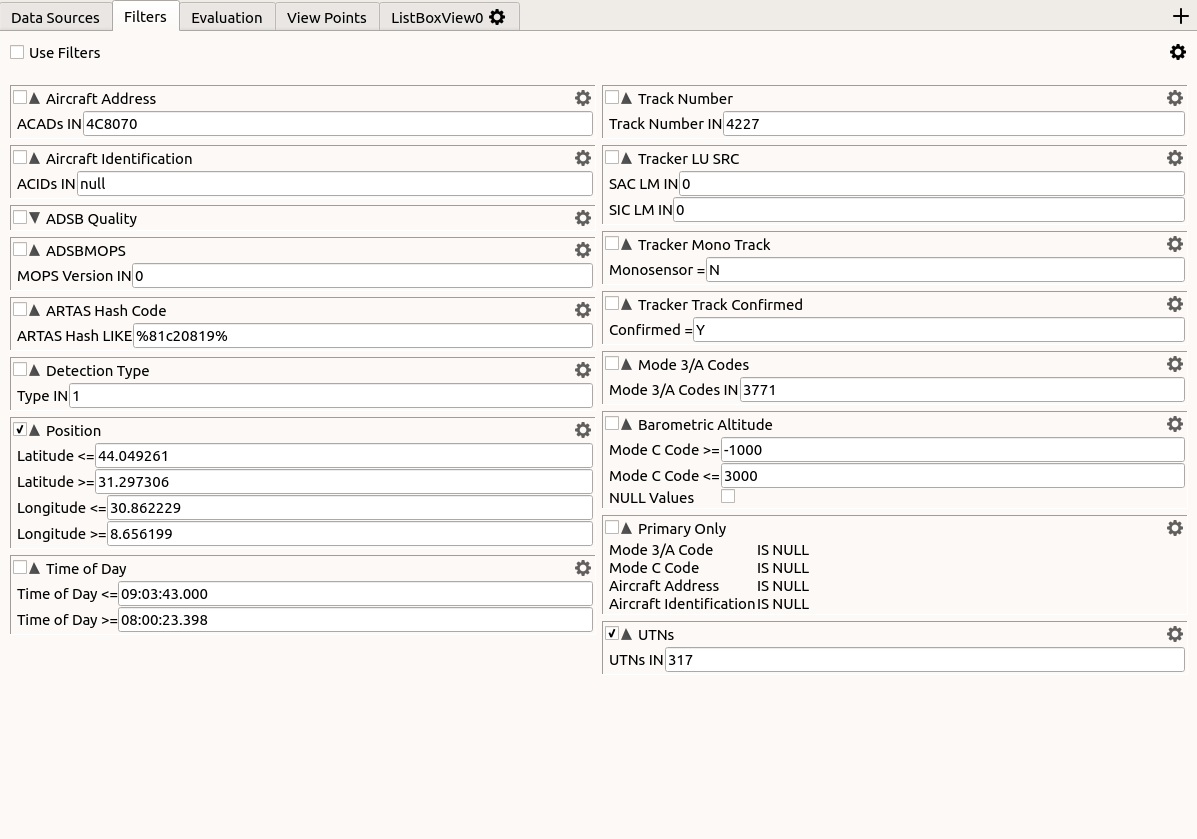
\includegraphics[width=19cm,frame]{figures/ui_filters.png}
  \caption{Filters Overview}
\end{figure}

At the top, the 'Use Filters' checkbox defines whether filtering is active. \\

Each filter consists of a checkbox, defining if a filter is active (contributes to the search query), a triangle-button (to show/hide the filter configuration elements), a unique name, and a manage button (activates a context menu). \\

Please \textbf{note} that the filter configuration will be saved at program shutdown, which is also true for new filters. At startup,  all filters from the configuration are generated and restored to their previous state. \\

Please also \textbf{note} that active filters, at the moment, are always combined with a logical AND. Therefore, when two filters  are active, only the intersection of data which both filters allow is loaded.

As an example, the 'Time of Day' filter limits the loaded data to a specific time window, to load only time slices of the dataset.  The 'Mode 3/A Codes' filter restricts to a list of (comma-separated) Mode 3/A codes, to single out specific flights. \\

For more information about filtering, please refer to section \nameref{sec:filtering}.
 
